\subsection{Модел с обобщена мрежа на производството на газови и полимерни продукти в нефтопреработвателна рафинерия}

\paragraph{Декларация за принос (съвместна публикация).}
\mbox{}\\
Настоящият раздел представя резултати, публикувани в съвместна статия \cite{Stratiev2023_1}.
Приносът на докторанта включва: (i) активно участие в съставянето на ОМ по описанието на процеса;
(ii) реализиране и провеждане на цялостната симулация чрез \textbf{\textit{OnlineGN}}, с което се верифицира моделът,
както и обработка/представяне на резултатите; (iii) подготовка и включване на всички фигури от симулациите и
описание на симулационния процес в текста на раздела.

В тази глава се представя ОМ модел на производството на газови и полимерни нефтопреработвателни продукти и неговата програмна симулация чрез \textit{OnlineGN}. Изграждането на модела и детайлите по формализацията са разгледани подробно в гореспомената статия ~\cite{Stratiev2023_1}.

\subsubsection{Увод в производството на продукти в нефтопреработвателна рафинерия}

\hspace*{2.5em}Моделирането на процесите на производство на рафинирани продукти в нефтопреработвателна рафинерия е полезен инструмент за производствено планиране, тъй като подпомага повишаването на ефективността и рентабилността на производството.

В литературата се срещат частични модели на разнообразните процеси в химическата индустрия и нефтопреработването. Например, в~\cite{Zhou2017} се разглежда оценка на риска в химическата индустрия; в~\cite{Infosys2018} се изследва интегрирането на инженерни модели с планови модели; в~\cite{40} се акцентира върху планирането в мащаб „цяла рафинерия“ при неопределеност в търсенето и цените на продуктите. Общата картина показва, че тези подходи третират отделни аспекти на проблема и по-рядко предлагат единна рамка, която да позволява едновременно описание, анализ и симулация на процесите като взаимосвързана система.

Подходът за моделиране на процесите в нефтопреработването чрез ОМ е оригинален, като публикациите в тази насока до момента са дело на част от авторите на~\cite{Stratiev2023_1}. Благодарение на високата изразителна мощ на ОМ, процесите могат да бъдат описани в детайл и да се отразят причинно--следствените зависимости чрез предикатите на преходите и характеристиките на ядрата. Това дава възможност да се обхванат едновременно структурата на процеса, логиката на протичането му и необходимата числова информация за анализ и симулация.

В предишни изследвания~\cite{87,88} е показано, че процесите на производство на автомобилен бензин~\cite{87} и дизелово гориво~\cite{88} в нефтопреработвателна рафинерия могат да бъдат моделирани чрез ОМ. Прегледът на литературата и досегашните резултати показват, че за цялостно представяне на производството на рафинирани продукти е необходимо постепенно да се моделират отделните технологични вериги и впоследствие да се обединят в обща йерархична структура. Апаратът на ОМ улеснява именно такова интегриране, тъй като отделни ОМ модели могат да бъдат трансформирани в подмрежи на по-общ модел.

Настоящата глава се фокусира върху моделирането и симулирането на производството на газово гориво, втечнен петролен газ (ВПГ, на англ. \textit{LPG}), пропилен и полипропилен, които са част от производствената верига за петролни газове, като допълнение към вече разгледаните процеси за автомобилен бензин и дизелово гориво. Целта е да се моделира разглежданата технологична верига в рамките на нефтопреработвателна рафинерия чрез ОМ, след което моделът да се симулира с \textit{OnlineGN} и да се потвърди неговата коректност.


\subsubsection{Технологична схема за производство на газово гориво, втечнен петролен газ, пропилен и полипропилен в нефтопреработвателна рафинерия}

\hspace*{2.5em}Технологичната производствена верига, използвана в рафинерията „ЛУКОЙЛ Нефтохим Бургас“ (ЛНБ) за производство на компонентите и крайните продукти -- газово гориво, втечнен петролен газ (ВПГ), пропилен и полипропилен, които са предмет на настоящото изследване, е представена на \textbf{Фигура~\ref{H}}.

\begin{figure}[H]
	\centering
	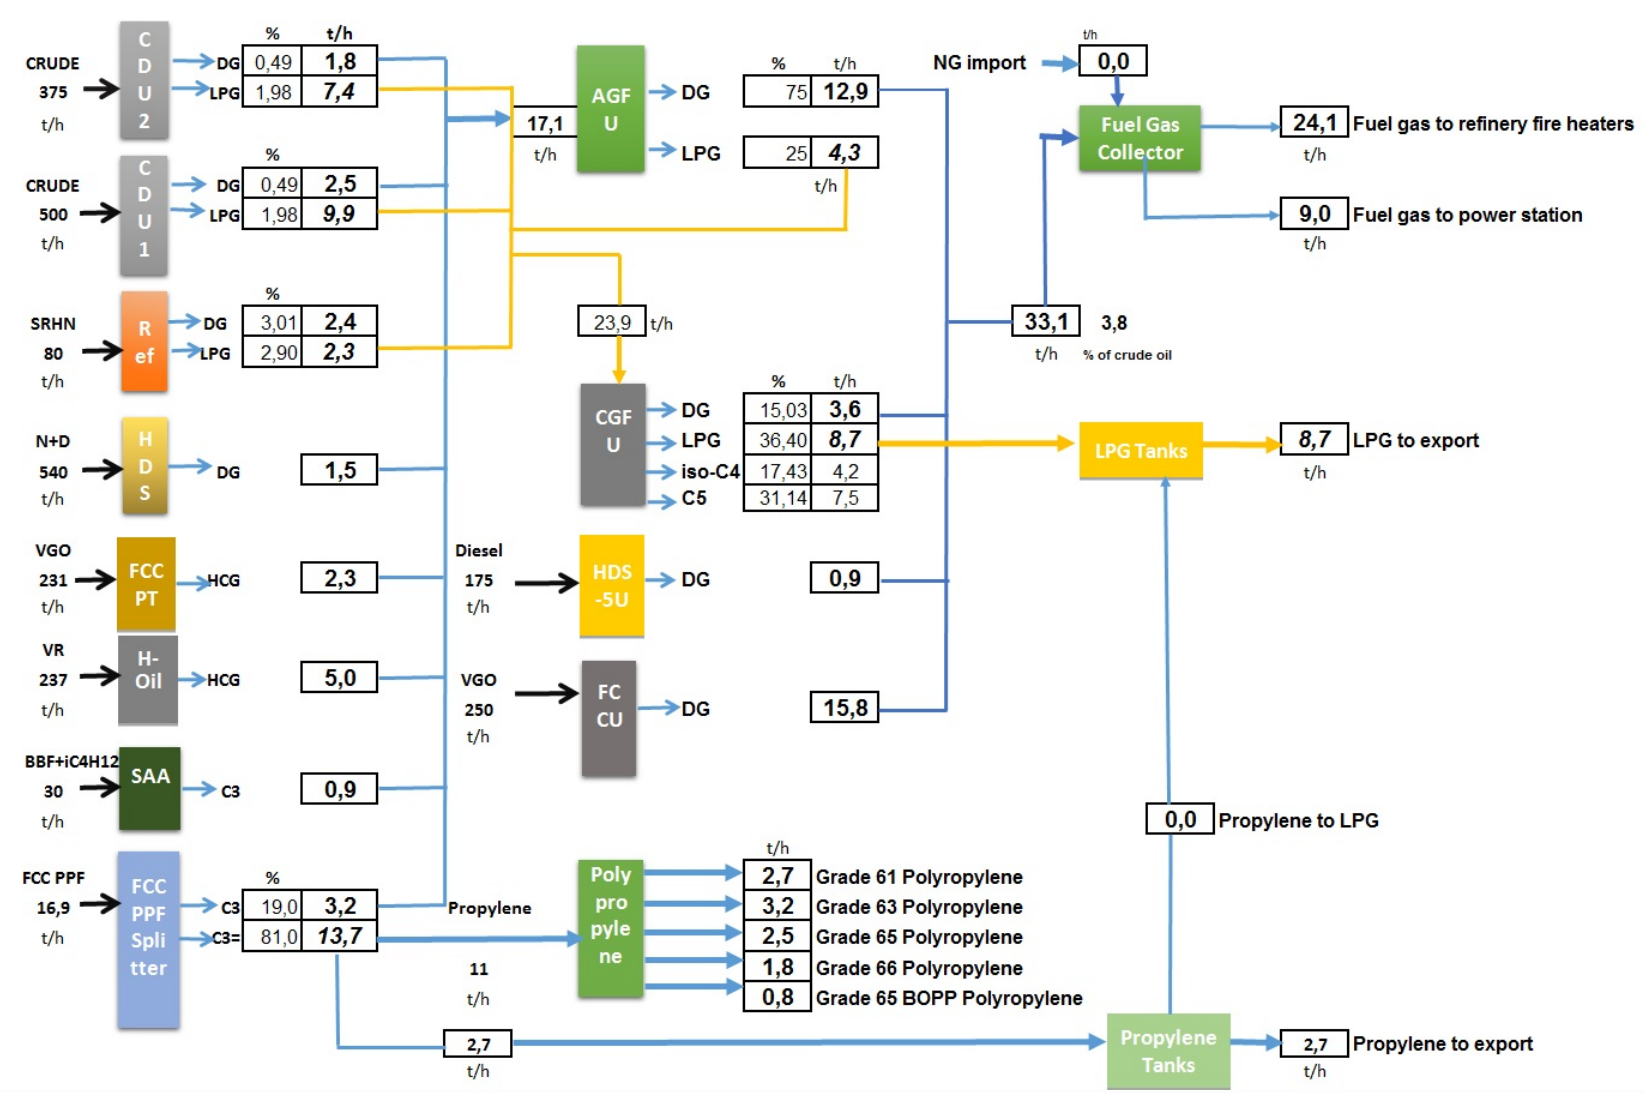
\includegraphics[scale=0.5]{4. applications/fuelGasEtc/images/Figure1.png}
	\caption{Технологична схема за производство на газово гориво, ВПГ, пропилен и полипропилен в нефтопреработвателна рафинерия.}
	\label{H}
\end{figure}

\noindent\textit{Легенда към \textbf{Фигура~\ref{H}} (пояснения на използваните съкращения):}
\begin{itemize}\setlength{\itemsep}{0pt}\setlength{\parskip}{0pt}
	\item \textit{CDU} -- инсталация за атмосферна дестилация на нефта и вакуумна дестилация на атмосферния остатък;
	\item \textit{Ref} -- инсталация за каталитичен реформинг;
	\item \textit{HDS} -- инсталация за хидроочистване на нефтени фракции;
	\item \textit{AGFU} -- инсталация за абсорбация и газофракциониране;
	\item \textit{CGFU} -- централна газофракционираща инсталация;
	\item \textit{HDS-5} -- хидроочистваща инсталация номер 5 от технологичната верига на изследваната рафинерия;
	\item \textit{SAA} -- алкилиране със сярна киселина;
	\item \textit{FCC PPF Splitter} -- ректификационна колона за разделяне на пропан-пропиленовата фракция на пропан и пропилен;
	\item \textit{Polypropylene} -- инсталация за производство на полипропилен чрез полимеризация на пропилен.
\end{itemize}

Тринадесет технологични инсталации в рафинерията участват в производствения процес на газово гориво, ВПГ, пропилен и полипропилен. Количествата на тези петролни газови продукти (в газова и течна фаза), извлечени от суровия нефт при процеса на атмосферна дестилация и генерирани в процесните инсталации -- риформер, хидроочистващи инсталации, \textit{FCC} и \textit{H-Oil} -- в резултат на химични реакции, зависят от произхода на суровия нефт и от експлоатационните режими в посочените инсталации. За случая, показан на \textbf{Фигура~\ref{H}}, производството на газово гориво възлиза на 3.8~\% от количеството суров нефт и повече от половината от него произхожда от флуидното каталитично крекиране (51.8~\%). Друг важен принос за производството на газово гориво има \textit{H-Oil} хидрокрекингът на вакуумен остатък в кипящ слой. Следователно производството на газово гориво е силно зависимо от строгостта на експлоатационните условия, прилагани и в двата процеса за преработка на тежки нефтени фракции -- \textit{FCC} и \textit{H-Oil}. 

Основният източник на ВПГ, както се вижда от данните на \textbf{Фигура~\ref{H}}, е дестилацията на суров нефт. Тя осигурява 75~\% от зареждането на Централната газофракционираща инсталация (\textit{CGFU}), където се извършва извличането на пропан и \textit{n}\,-бутан; тяхното смесване формира рафинирания продукт ВПГ. От \textbf{Фигура~\ref{H}} се вижда, че производството на ВПГ е приблизително четири пъти по-малко от това на газовото гориво. Данните на \textbf{Фигура~\ref{H}} показват, че ако количеството газово гориво е недостатъчно за покриване на енергийните нужди на рафинерията, съществува възможност за внос на природен газ за допълване на наличностите от газово гориво. 

В зависимост от пазарните изисквания течният пропилен може да се експортира като химически сорт за полимеризационен пропилен или да се използва като компонент на продукта ВПГ. Обикновено от инсталацията за полипропилен се произвеждат и изнасят шест сорта полипропиленови продукти.


\subsubsection{Основни резултати: обобщеномрежов модел}

\hspace*{2.5em}ОМ на \textbf{Фигура~\ref{fig3}} съдържа 17 прехода, 55 позиции и 47 типа ядра, съответстващи на следните потоци, продукти и процесни звена:
\begin{itemize}
	\item[$\sigma_1$] ― суров нефт, преработван в \textit{CDU-2}, \textit{t/h}
	\item[$\sigma_2$] ― суров нефт, преработван в \textit{CDU-1}, \textit{t/h}
	\item[$\sigma_3$] ― нафта от пряка дестилация, преработвана в инсталацията за каталитичен реформинг, \textit{t/h}
	\item[$\sigma_4$] ― нафтови и дизелови фракции, преработвани в инсталации за хидрообработка (хидроочистване), \textit{t/h}
	\item[$\sigma_5$] ― вакуумен газьол, преработван в инсталация за хидроочистване на суровината за флуиден каталитичен крекинг (\textit{FCC}), \textit{t/h}
	\item[$\sigma_6$] ― вакуумен остатък, преработван в инсталация за хидрокрекинг по технология \textit{H-Oil}, \textit{t/h}
	\item[$\sigma_7$] ― бутан-бутиленова фракция и изобутен за алкилиране със сярна киселина, \textit{t/h}
	\item[$\sigma_8$] ― пропан-пропиленова фракция от \textit{FCC} за разделяне на пропан и пропилен, \textit{t/h}
	\item[$\sigma_9$] ― първичен и вторичен дизел за хидроочистване в инсталацията \textit{HDS-5}, \textit{t/h}
	\item[$\sigma_{10}$] ― хидроочистен вакуумен газьол и вакуумен газьол от \textit{H-Oil} за преработка във флуиден каталитичен крекинг (\textit{FCC}), \textit{t/h}
	\item[$\sigma_{11}$] ― вносен природен газ за допълване на горивния газ при високо потребление, \textit{t/h}
	
	\item[$\rho_1$] ― инсталация за атмосферна (първична) дестилация на суров нефт \textit{(CDU-2)}
	\item[$\rho_2$] ― инсталация за атмосферна (първична) дестилация на суров нефт \textit{(CDU-1)}
	\item[$\rho_3$] ― инсталация за каталитичен реформинг (каталитичен реформер)
	\item[$\rho_4$] ― инсталации за хидроочистване на нафтови и дизелови фракции
	\item[$\rho_5$] ― инсталация за хидроочистване на суровината за \textit{FCC} (\textit{FCC feed hydrotreater})
	\item[$\rho_6$] ― инсталация за хидрокрекинг на вакуумен остатък по технология \textit{H-Oil}
	\item[$\rho_7$] ― инсталация за алкилиране със сярна киселина
	\item[$\rho_8$] ― инсталация за разделяне на пропан-пропиленова фракция от \textit{FCC} (\textit{FCC PPF splitter})
	\item[$\rho_9$] ― инсталация за абсорбация и газофракциониране (\textit{AGFU})
	\item[$\rho_{10}$] ― междинен резервоар за \textit{LPG} (ВПГ) за събиране на суровина за централната газофракционираща инсталация (\textit{CGFU})
	\item[$\rho_{11}$] ― инсталация за хидроочистване на дизелово гориво \textit{(HDS-5)}
	\item[$\rho_{12}$] ― инсталация за флуиден каталитичен крекинг (\textit{FCC})
	\item[$\rho_{13}$] ― централна газофракционираща инсталация (\textit{CGFU})
	\item[$\rho_{14}$] ― резервоарен парк за \textit{LPG} (ВПГ)
	\item[$\rho_{15}$] ― резервоарен парк за горивен газ
	
	\item[$\alpha_1$] ― ВПГ (\textit{LPG}) продукт от \textit{CDU-2}, \textit{t/h}
	\item[$\alpha_2$] ― ВПГ (\textit{LPG}) продукт от \textit{CDU-1}, \textit{t/h}
	\item[$\alpha_3$] ― ВПГ (\textit{LPG}) продукт от инсталацията за каталитичен реформинг, \textit{t/h}
	\item[$\alpha_4$] ― ВПГ (\textit{LPG}) продукт от \textit{AGFU}, \textit{t/h}
	\item[$\alpha_5$] ― суровина за \textit{CGFU}, \textit{t/h}
	\item[$\alpha_6$] ― ВПГ (\textit{LPG}) продукт от \textit{CGFU} към резервоарния парк, \textit{t/h}
	
	\item[$\beta$]  ― горивен газ за захранване на \textit{AGFU}, \textit{t/h}
	\item[$\beta_1$] ― горивен газ продукт от \textit{CDU-2}, \textit{t/h}
	\item[$\beta_2$] ― горивен газ продукт от \textit{CDU-1}, \textit{t/h}
	\item[$\beta_3$] ― горивен газ продукт от инсталацията за каталитичен реформинг, \textit{t/h}
	\item[$\beta_4$] ― горивен газ продукт от инсталациите за хидроочистване на нафтови и дизелови фракции, \textit{t/h}
	\item[$\beta_5$] ― горивен газ продукт от инсталацията за хидроочистване на суровината за \textit{FCC}, \textit{t/h}
	\item[$\beta_6$] ― горивен газ продукт от инсталацията \textit{H-Oil} за хидрокрекинг на вакуумен остатък, \textit{t/h}
	\item[$\beta_7$] ― пропанова фракция от инсталацията за алкилиране със сярна киселина, \textit{t/h}
	\item[$\beta_8$] ― сух горивен газ продукт от \textit{AGFU}, \textit{t/h}
	\item[$\beta_9$] ― сух горивен газ продукт от \textit{CGFU}, \textit{t/h}
	\item[$\beta_{10}$] ― сух горивен газ продукт от \textit{HDS-5}, \textit{t/h}
	\item[$\beta_{11}$] ― сух горивен газ продукт от \textit{FCC}, \textit{t/h}
	
	\item[$\gamma_1$] ― пропан продукт от \textit{FCC PPF splitter}, \textit{t/h}
	\item[$\gamma_2$] ― пропиленов продукт от \textit{FCC PPF splitter} за захранване на инсталация за полипропилен, \textit{t/h}
	\item[$\gamma_3$] ― пропиленов продукт от \textit{FCC PPF splitter}, \textit{t/h}
	
	\item[$\delta_1$] ― полипропилен, марка 61 (висок индекс на топене), \textit{t/h}
	\item[$\delta_2$] ― полипропилен, марка 63 (висок индекс на топене), \textit{t/h}
	\item[$\delta_3$] ― полипропилен, марка 65 (висок индекс на топене), \textit{t/h}
	\item[$\delta_4$] ― полипропилен, марка 66 (висок индекс на топене), \textit{t/h}
	\item[$\delta_5$] ― полипропилен, марка 65 \textit{BOPP} (висок индекс на топене), \textit{t/h}
	
	\item[$\epsilon_1$] ― ВПГ (\textit{LPG}) продукт за износ, \textit{t/h}
	\item[$\epsilon_2$] ― горивен газ продукт за захранване на електроцентралата на рафинерията, \textit{t/h}
	\item[$\epsilon_3$] ― горивен газ продукт за захранване на процесните пещи на рафинерията, \textit{t/h}
\end{itemize}

\vspace*{-0.85em}

$$Z_1 = \langle\{l_1, l_{11} \}, \{l_{9}, l_{10}, l_{11} \},
\begin{array}{c|ccc}
	& l_{9} & l_{10} & l_{11} \\ \hline
	l_{1}  & false & false & true \\
	l_{11}  & W_{11,9} & W_{11,10} & true
\end{array} \rangle,$$
където: \\
$W_{11,9} = $ „има заявка за продукт ВПГ от \textit{CDU-2}“;\\
$W_{11,10} = $ „има заявка за продукт горивен газ от \textit{CDU-2}“; 

\vspace{0.10cm}

\noindent
Ядрото $\sigma_1$ влиза в позиция $l_{11}$ и се обединява с ядрото $\rho_1$, получавайки характеристика:
$$„\mbox{текущо количество суров петрол в \textit{CDU-2}}“.$$

\vspace{-0.5em}

В следващата времева стъпка ядрото $\rho_1$ се разделя на три ядра - самото $\rho_1$, което остава в $l_{11}$, и ядрата $\alpha_1$ и $\beta_1$.

Ядрото $\alpha_1$ получава характеристика:
$$„\mbox{текущо количество ВПГ продукт от \textit{CDU-2}}“$$
в позиция $l_{9}$, ядрото $\beta_1$ - характеристика:
$$„\mbox{текущо количество горивен газ от \textit{CDU-2}}“$$
в позиция $l_{10}$, а ядрото $\rho_1$ запазва характеристика:
$$„\mbox{текущо количество суров петрол в \textit{CDU-2}}“.\vspace{-0.95em}$$


$$Z_2 = \langle\{l_2, l_{14} \}, \{l_{12}, l_{13}, l_{14} \},
\begin{array}{c|ccc}
	& l_{12} & l_{13} & l_{14} \\ \hline
	l_{2}  & false & false & true \\
	l_{14}  & W_{14,12} & W_{14,13} & true
\end{array} \rangle,$$
където:\\
$W_{14,12} =~$„има заявка за продукт ВПГ от \textit{CDU-1}“;\\
$W_{14,13} =~$„има заявка за продукт горивен газ от \textit{CDU-1}“.

\vspace{0.10cm}

\noindent
Ядрото $\sigma_2$ влиза в позиция $l_{14}$ и се обединява с ядро $\rho_2$, получавайки характеристика:
$$„\mbox{текущо количество суров петрол в \textit{CDU-1}}“.$$

\vspace{-0.5em}

В следващата времева стъпка ядрото $\rho_2$ се разделя на три ядра - самото $\rho_2$, което остава в $l_{14}$, и ядрата $\alpha_2$ и $\beta_2$.

Ядрото $\alpha_2$ получава характеристика:
$$„\mbox{текущо количество ВПГ продукт от \textit{CDU-1}}“$$
в позиция $l_{12}$, ядрото $\beta_2$ - характеристика:
$$„\mbox{текущо количество горивен газ от \textit{CDU-1}}“$$
в позиция $l_{13}$, а ядрото $\rho_2$ запазва характеристика:
$$„\mbox{текущо количество суров петрол в \textit{CDU-1}}“. \vspace{-0.95em}$$


$$Z_3 = \langle\{l_3, l_{17} \}, \{l_{15}, l_{16}, l_{17} \},
\begin{array}{c|ccc}
	& l_{15} & l_{16} & l_{17} \\ \hline
	l_{3}  & false & false & true \\
	l_{17}  & W_{17,15} & W_{17,16} & true
\end{array} \rangle,$$
където:\\
$W_{17,15} =~$„има заявка за продукт ВПГ от каталитичния реформер“;\\
$W_{17,16} =~$„има заявка за продукт горивен газ от каталитичния реформер“.

\vspace{0.10cm}

\noindent
Ядрото $\sigma_3$ влиза в позиция $l_{17}$ и се обединява с ядро $\rho_3$, получавайки характеристика:
$$„\mbox{текущо количество нафта в каталитичния реформер}“.$$

\vspace{-0.5em}

В следващата времева стъпка ядрото $\rho_3$ се разделя на три ядра - самото $\rho_3$, което остава в $l_{17}$, и ядрата $\alpha_3$ и $\beta_3$.

Ядрото $\alpha_3$ получава характеристика:
$$„\mbox{текущо количество ВПГ продукт от каталитичния реформер}“$$
в позиция $l_{15}$, ядрото $\beta_3$ - характеристика:
$$„\mbox{текущо количество горивен газ от каталитичния реформер}“$$
в позиция $l_{16}$, а ядрото $\rho_3$ запазва характеристика:
$$„\mbox{текущо количество нафта в каталитичния реформер}“. \vspace{-0.95em}$$


$$Z_4 = \langle\{l_4, l_{19} \}, \{l_{18}, l_{19} \},
\begin{array}{c|cc}
	& l_{18} & l_{19} \\ \hline
	l_{4}  & false & true \\
	l_{19}  & W_{19,18} & true
\end{array} \rangle,$$
където:\\
$W_{19,18} =~$„има заявка за продукт горивен газ от нафтовите и дизелови хидроочистватели“.

\begin{figure}[H]
	\centering
	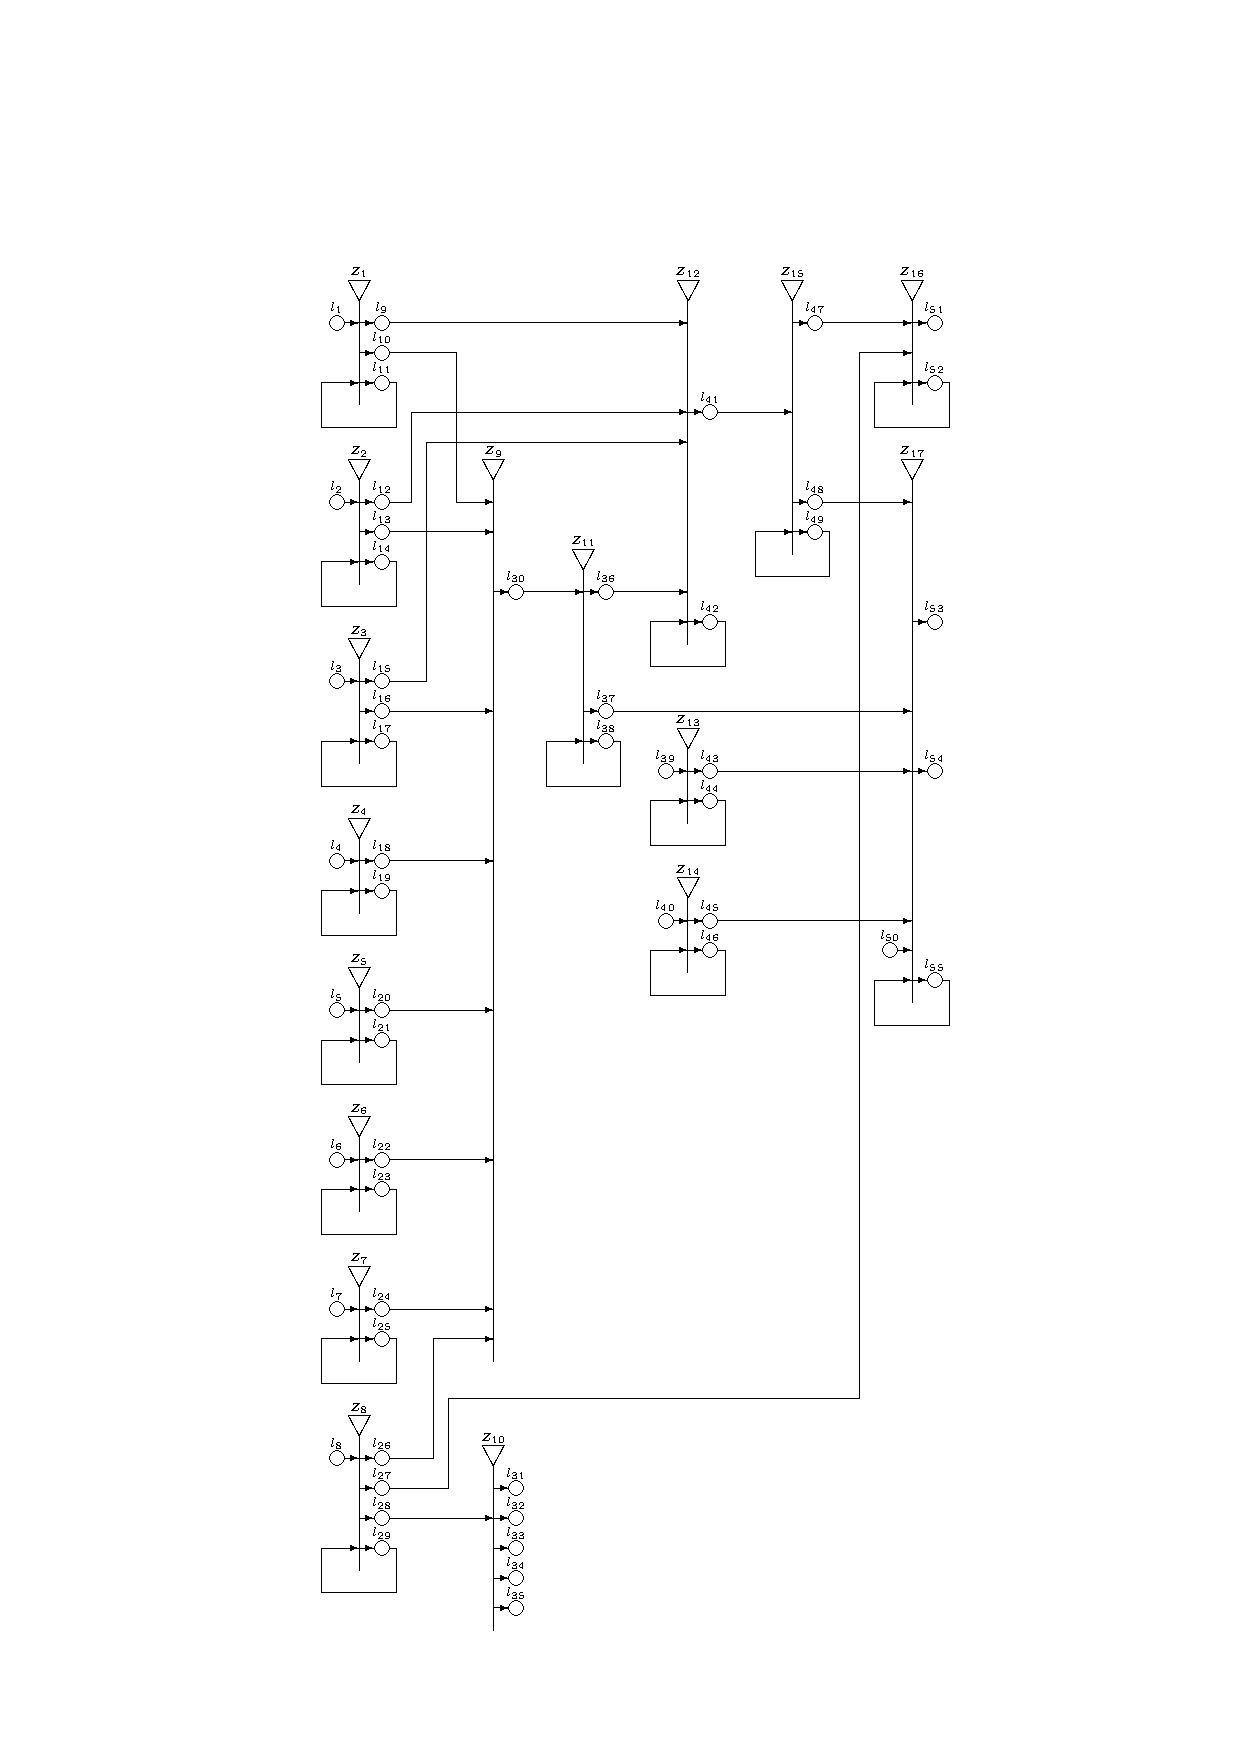
\includegraphics[width=10.3cm]{4. applications/fuelGasEtc/images/Figure3.pdf}
	\caption{ОМ модел.}
	\label{fig3}
\end{figure}


\noindent
Ядрото $\sigma_4$ влиза в позиция $l_{19}$ и се обединява с ядрото $\rho_4$, получавайки характеристика:
$$„\mbox{текущо количество нафта и дизел в нафтовите и дизелови хидроочистватели}“.$$

\vspace{-0.5em}

В следващата времева стъпка ядрото $\rho_4$ се разделя на две ядра - самото $\rho_4$, което остава в $l_{19}$, и ядрото $\beta_4$.

Ядрото $\beta_4$ получава характеристика:
$$„\mbox{текущо количество горивен газ от нафтовите и дизелови хидроочистватели}“$$
в позиция $l_{18}$, а ядрото $\rho_4$ запазва характеристика:
$$„\mbox{текущо количество нафта и дизел в нафтовите и дизелови хидроочистватели}“.$$

\vspace{-0.3em}

$$Z_5 = \langle\{l_5, l_{21} \}, \{l_{20}, l_{21} \},
\begin{array}{c|cc}
	& l_{20} & l_{21} \\ \hline
	l_{5}  & false & true \\
	l_{21}  & W_{21,20} & true
\end{array} \rangle,$$
където:\\
$W_{21,20} =~$„има заявка за продукт горивен газ от хидроочиствателя на хранилка за \textit{FCC}“.

\vspace{0.10em}

\noindent
Ядрото $\sigma_5$ влиза в позиция $l_{21}$ и се обединява с ядрото $\rho_5$, получавайки характеристика:
$$„\mbox{текущо количество вакуумен газьол в хидроочиствателя на хранилка за \textit{FCC}}“.$$

\vspace{-0.5em}

В следващата времева стъпка ядрото $\rho_5$ се разделя на две ядра - самото $\rho_5$, което остава в $l_{21}$, и ядрото $\beta_5$.

Ядрото $\beta_5$ получава характеристика:
$$„\mbox{текущо количество горивен газ в хидроочиствателя на хранилка за \textit{FCC}}“$$
в позиция $l_{20}$, а ядрото $\rho_5$ запазва характеристика:
$$„\mbox{текущо количество вакуумен газьол в хидроочиствателя на хранилка за \textit{FCC}}“.$$

\vspace{-0.3em}

$$Z_6 = \langle\{l_6, l_{23} \}, \{l_{22}, l_{23} \},
\begin{array}{c|cc}
	& l_{22} & l_{23} \\ \hline
	l_{6}  & false & true \\
	l_{23}  & W_{23,22} & true
\end{array} \rangle,$$
където:\\
$W_{23,22} =~$„има заявка за продукт горивен газ от \textit{H-Oil}“.

\vspace{0.1em}

\noindent
Ядрото $\sigma_6$ влиза в позиция $l_{23}$ и се обединява с ядрото $\rho_6$, получавайки характеристика:
$$„\mbox{текущо количество вакуумен остатък в \textit{H-Oil}}“.$$

\vspace{-0.5em}

В следващата времева стъпка ядрото $\rho_6$ се разделя на две ядра - самото $\rho_6$, което остава в $l_{23}$, и ядрото $\beta_6$.

Ядрото $\beta_6$ получава характеристика:
$$„\mbox{текущо количество горивен газ от \textit{H-Oil}}“$$
в позиция $l_{22}$, а ядрото $\rho_6$ запазва характеристика:
$$„\mbox{текущо количество вакуумен остатък в \textit{H-Oil}}“.$$
\vspace{-0.3em}
$$Z_7 = \langle\{l_7, l_{25} \}, \{l_{24}, l_{25} \},
\begin{array}{c|cc}
	& l_{24} & l_{25} \\ \hline
	l_{7}  & false & true \\
	l_{25}  & W_{25,24} & true
\end{array} \rangle,$$
където:\\
$W_{25,24} =~$„има заявка за продукт пропанова фракция от алкилирането със сярна киселина“.

\vspace{0.1em}

\noindent
Ядрото $\sigma_7$ влиза в позиция $l_{25}$ и се обединява с ядро $\rho_7$, получавайки характеристика:
$$„\mbox{текущо количество бутан-бутиленова фракция и изобутан в алкилирането със сярна киселина}“.$$
\vspace{-0.5em}
В следващата времева стъпка ядрото $\rho_7$ се разделя на две ядра - самото $\rho_7$, което остава в $l_{25}$, и ядро $\beta_{7}$.

Ядрото $\beta_{7}$ получава характеристика:
$$„\mbox{текущо количество пропанова фракция в алкилирането със сярна киселина}“$$
в позиция $l_{24}$, а ядрото $\rho_7$ запазва характеристика:
$$„\mbox{текущо количество бутан-бутиленова фракция и изобутан в алкилирането със сярна киселина}“.$$
\vspace{-0.3em}
$$Z_8 = \langle\{l_8, l_{29} \}, \{l_{26}, l_{27}, l_{28}, l_{29} \},
\begin{array}{c|cccc}
	& l_{26} & l_{27} & l_{28} & l_{29} \\ \hline
	l_{8}  & false & false & false & true \\
	l_{29}  & W_{29,26} & W_{29,27} & W_{29,28} & true
\end{array} \rangle,$$
където:\\
$W_{29,26} =~$„има заявка за пропанов продукт от \textit{FCC PPF splitter} за производство на ВПГ“;\\
$W_{29,27} =~$„има заявка за пропилен за полимеризация от \textit{FCC PPF splitter}“;\\
$W_{29,28} =~$„има заявка за пропиленов продукт от \textit{FCC PPF splitter} за износ“.

\vspace{0.1em}

\noindent
Ядрото $\sigma_8$ влиза в позиция $l_{29}$ и се обединява с ядро $\rho_8$, получавайки характеристика:
$$„\mbox{текущо количество \textit{FCC PPF} във \textit{FCC PPF splitter}}“.$$

\vspace{-0.5em}

В следващата времева стъпка ядрото $\rho_8$ се разделя на четири ядра - самото $\rho_8$, което остава в $l_{29}$, и ядрата $\gamma_{1}$, $\gamma_{2}$ и $\gamma_{3}$.

Ядрата $\gamma_{1}$, $\gamma_{2}$ и $\gamma_{3}$ получават съответно характеристики:
$$„\mbox{текущо количество пропанов продукт във \textit{FCC PPF splitter}}“$$
в позиция $l_{26}$,
$$„\mbox{текущо количество пропиленов продукт за полимеризация във \textit{FCC PPF splitter}}“$$
в позиция $l_{27}$,
$$„\mbox{текущо количество пропиленов продукт за износ във \textit{FCC PPF splitter}}“$$
в позиция $l_{28}$, а ядрото $\rho_8$ запазва характеристика:
$$„\mbox{текущо количество \textit{FCC PPF} във \textit{FCC PPF splitter}}“.$$

\vspace{-0.3em}

$$Z_9 = \langle\{l_{10}, l_{13}, l_{16}, l_{18}, l_{20}, l_{22}, l_{24}, l_{26}\}, \{l_{30}\},
\begin{array}{c|c}
	& l_{30} \\ \hline
	l_{10} & true \\
	l_{13} & true \\
	l_{16} & true \\
	l_{18} & true \\
	l_{20} & true \\
	l_{22} & true \\
	l_{24} & true \\
	l_{26} & true
\end{array} \rangle.$$

\noindent
Всички $\beta$-ядра се обединяват в позиция $l_{30}$ в едно ядро $\beta$ с характеристика:
$$„\mbox{текущо количество горивен газ - захранване за \textit{AGFU}}“.$$

\vspace{-0.3em}

$$Z_{10} = \langle\{l_{28}\}, \{l_{31}, l_{32}, l_{33}, l_{34}, l_{35}\},
\begin{array}{c|ccccc}
	& l_{31} & l_{32} & l_{33} & l_{34} & l_{35} \\ \hline
	l_{28} & W_{28,31} & W_{28,32} & W_{28,33} & W_{28,34} & W_{28,35}
\end{array} \rangle,$$
където:\\
$W_{28,31} =~$„има заявка за полипропилен, клас 61 (висок индекс на топене), от полипропиленовата установка“;\\
$W_{28,32} =~$„има заявка за полипропилен, клас 63 (висок индекс на топене), от полипропиленовата установка“;\\
$W_{28,33} =~$„има заявка за полипропилен, клас 65 (висок индекс на топене), от полипропиленовата установка“;\\
$W_{28,34} =~$„има заявка за полипропилен, клас 66 (висок индекс на топене), от полипропиленовата установка“;\\
$W_{28,35} =~$„има заявка за полипропилен, клас 66 \textit{BOPP} (висок индекс на топене), от полипропиленовата установка“.

\vspace{0.1em}

\noindent
Ядрото $\gamma_2$ се разделя на пет ядра $\delta_1,\dots,\delta_5$, които получават характеристики:
$$„\mbox{текущо количество полипропилен, клас 61, от полипропиленовата установка}“$$
в позиция $l_{31}$,
$$„\mbox{текущо количество полипропилен, клас 63, от полипропиленовата установка}“$$
в позиция $l_{32}$,
$$„\mbox{текущо количество полипропилен, клас 65, от полипропиленовата установка}“$$
в позиция $l_{33}$,
$$„\mbox{текущо количество полипропилен, клас 66, от полипропиленовата установка}“$$
в позиция $l_{34}$,
$$„\mbox{текущо количество полипропилен, клас 65 \textit{BOPP}, от полипропиленовата установка}“$$
в позиция $l_{35}$.

\vspace{-0.3em}

$$Z_{11} = \langle\{l_{30}, l_{38}\}, \{l_{36}, l_{37}, l_{38}\},
\begin{array}{c|ccc}
	& l_{36} & l_{37} & l_{38} \\ \hline
	l_{30} & false & false & true \\
	l_{38} & W_{38,36} & W_{38,37} & true
\end{array} \rangle,$$
където:\vspace{-0.3em}\\
$W_{38,36} =~$„има заявка за продукт ВПГ от \textit{AGFU}“;\\
$W_{38,37} =~$„има заявка за продукт горивен газ от \textit{AGFU}“.

\vspace{0.1em}

\noindent
Ядрото $\beta$ влиза в позиция $l_{38}$ и се обединява с ядро $\rho_9$, получавайки характеристика:
$$„\mbox{текущо количество горивен газ - захранване на \textit{AGFU}}“.$$

\vspace{-0.5em}

В следващата времева стъпка ядрото $\rho_9$ се разделя на три ядра - самото $\rho_9$, което остава в $l_{38}$, и ядрата $\alpha_4$ и $\beta_8$.

Ядрото $\alpha_4$ получава характеристика:
$$„\mbox{текущо количество ВПГ продукт от \textit{AGFU}}“$$
в позиция $l_{36}$, а ядрото $\beta_8$ - характеристика:
$$„\mbox{текущо количество горивен газ от \textit{AGFU}}“$$
в позиция $l_{37}$.

\vspace{0.1em}

$$Z_{12} = \langle\{l_{9}, l_{12}, l_{15}, l_{36}, l_{42}\}, \{l_{41}, l_{42}\},
\begin{array}{c|cc}
	& l_{41} & l_{42} \\ \hline
	l_{9}  & false & true \\
	l_{12} & false & true \\
	l_{15} & false & true \\
	l_{36} & false & true \\
	l_{42} & true  & true
\end{array} \rangle.$$

\textls[-20]{Всички $\alpha$-ядра ($\alpha_1,\alpha_2,\alpha_3,\alpha_4$) се обединяват в позиция $l_{42}$ с ядро $\rho_{10}$ и получават характеристика}:
$$„\mbox{текущо количество ВПГ захранване, съхранявано в резервоар за \textit{CGFU}}“.$$

\vspace{-0.5em}

В следващата времева стъпка ядрото $\rho_{10}$ се разделя на две ядра - самото $\rho_{10}$, което остава в $l_{42}$, и ядро $\alpha_5$, което влиза в позиция $l_{41}$ с характеристика:
$$„\mbox{текущо количество ВПГ захранване за \textit{CGFU}}“.$$

$$Z_{13} = \langle\{l_{39}, l_{44}\}, \{l_{43}, l_{44}\},
\begin{array}{c|cc}
	& l_{43} & l_{44} \\ \hline
	l_{39} & false & true \\
	l_{44} & W_{44,43} & true
\end{array} \rangle,$$
където:\\
$W_{44,43} =~$„има заявка за продукт горивен газ от \textit{HDS-5}“.

\vspace{0.1em}

\noindent
Ядрото $\sigma_9$ влиза в позиция $l_{44}$ и се обединява с ядро $\rho_{11}$, получавайки характеристика:
$$„\mbox{текущо количество първичен и вторичен дизел -- захранване за \textit{HDS-5}}“.$$

\vspace{-0.5em}

В следващата времева стъпка ядрото $\rho_{11}$ се разделя на две ядра - самото $\rho_{11}$, което остава в $l_{44}$ и запазва характеристика:
$$„\mbox{текущо количество първичен и вторичен дизел -- захранване за \textit{HDS-5}}“$$
и ядро $\beta_{10}$, което влиза в позиция $l_{43}$ с характеристика:
$$„\mbox{текущо количество сух горивен газ в \textit{HDS-5}}“.$$

\vspace{-0.3em}

$$Z_{14} = \langle\{l_{40}, l_{46}\}, \{l_{45}, l_{46}\},
\begin{array}{c|cc}
	& l_{45} & l_{46} \\ \hline
	l_{40} & false & true \\
	l_{46} & W_{46,45} & true
\end{array} \rangle,$$
където:\\
$W_{46,45} =~$„има заявка за продукт горивен газ от \textit{FCCU}“.

\vspace{0.1em}

\noindent
Ядрото $\sigma_{10}$ влиза в позиция $l_{46}$ и се обединява с ядро $\rho_{12}$, получавайки характеристика:
$$„\mbox{текущо количество хидроочистен вакуумен газьол -- захранване за \textit{FCCU}}“.$$

\vspace{-0.5em}

В следващата времева стъпка ядрото $\rho_{12}$ се разделя на две ядра -- самото $\rho_{12}$, което остава в $l_{46}$ и запазва характеристика:
$$„\mbox{текущо количество хидроочистен вакуумен газьол - захранване за \textit{FCCU}}“$$
и ядро $\beta_{11}$, което влиза в позиция $l_{45}$ с характеристика:
$$„\mbox{текущо количество сух горивен газ във \textit{FCCU}}“.$$

\vspace{-0.3em}

$$Z_{15} = \langle\{l_{41}, l_{49}\}, \{l_{47}, l_{48}, l_{49}\},
\begin{array}{c|ccc}
	& l_{47} & l_{48} & l_{49} \\ \hline
	l_{41} & false & false & true \\
	l_{49} & W_{49,47} & W_{49,48} & true
\end{array} \rangle,$$
където:\\
$W_{49,47} =~$„има заявка за продукт ВПГ от \textit{CGFU}“;\\
$W_{49,48} =~$„има заявка за продукт горивен газ от \textit{CGFU}“.

\vspace{0.1em}

\noindent
Ядрото $\alpha_5$ влиза в позиция $l_{49}$ и се обединява с ядро $\rho_{13}$, получавайки характеристика:
$$„\mbox{текущо количество ВПГ захранване в \textit{CGFU}}“.$$

\vspace{-0.5em}

В следващата времева стъпка ядрото $\rho_{13}$ се разделя на три ядра -- самото $\rho_{13}$, което остава в $l_{49}$, и ядрата $\alpha_6$ и $\beta_9$.

Ядрото $\alpha_6$ получава характеристика:
$$„\mbox{текущо количество ВПГ продукт от \textit{CGFU}}“$$
в позиция $l_{47}$, а ядрото $\beta_9$ - характеристика:
$$„\mbox{текущо количество горивен газ от \textit{CGFU}}“$$
в позиция $l_{48}$.

\vspace{-0.3em}

$$Z_{16} = \langle\{l_{27}, l_{47}, l_{52}\}, \{l_{51}, l_{52}\},
\begin{array}{c|cc}
	& l_{51} & l_{52} \\ \hline
	l_{27} & false & true \\
	l_{47} & false & true \\
	l_{52} & true  & true
\end{array} \rangle.$$

Ядрата $\alpha_6$ и $\gamma_2$ влизат в позиция $l_{52}$ и се обединяват с ядро $\rho_{14}$, получавайки характеристика:
$$„\mbox{текущо количество ВПГ в парковата площадка за ВПГ за износ}“.$$

\vspace{-0.5em}

В следващата времева стъпка ядрото $\rho_{14}$ се разделя на две ядра - самото $\rho_{14}$ и ядро $\varepsilon_1$, което влиза в позиция $l_{51}$ с характеристика:
$$„\mbox{текущо количество ВПГ, изпратен за износ}“.$$

\vspace{-0.3em}

$$Z_{17} = \langle\{l_{37}, l_{43}, l_{45}, l_{48}, l_{50}, l_{55}\}, \{l_{53}, l_{54}, l_{55}\},
\begin{array}{c|ccc}
	& l_{53} & l_{54} & l_{55} \\ \hline
	l_{37} & false & false & true \\
	l_{43} & false & false & true \\
	l_{45} & false & false & true \\
	l_{48} & false & false & true \\
	l_{50} & false & false & true \\
	l_{55} & W_{55,53} & W_{55,54} & false
\end{array} \rangle,$$
където:\\
$W_{55,53} =~$„има заявка за продукт горивен газ за електроцентралата на рафинерията“;\\
$W_{55,54} =~$„има заявка за продукт горивен газ за процесните пещи на рафинерията“.

\vspace{0.1em}

\textls[-20]{Ядрата $\beta_8, \beta_9, \sigma_9, \sigma_{10}, \sigma_{11}$ влизат в позиция $l_{55}$ и се обединяват с ядро $\rho_{15}$, получавайки характеристика}:
$$„\mbox{текущо количество горивен газ}“.$$

Ядрото $\rho_{15}$ се разделя на три ядра -- самото $\rho_{15}$, което остава в $l_{55}$, и ядрата $\varepsilon_2$ и $\varepsilon_3$.

Ядрото $\varepsilon_2$ получава характеристика:
$$„\mbox{текущо количество горивен газ за електроцентралата на рафинерията}“$$
в позиция $l_{53}$, а ядрото $\varepsilon_3$ -- характеристика:
$$„\mbox{текущо количество горивен газ за процесните пещи на рафинерията}“$$
в позиция $l_{54}$.

\subsubsection{Бележки по резултатите и обобщеномрежов модел}

\hspace*{2.5em}Производството на газово гориво, ВПГ, пропилен и полипропилен в рафинерия представлява сложен паралелен процес, включващ множество технологични инсталации, които могат да доставят променливи количества от тези продукти в зависимост от суровинния състав (\textit{crude slate}), активността и селективността на използвания катализатор и експлоатационните режими в отделните инсталации. Установено е, че този процес може да бъде адекватно представен чрез ОМ.

Разработеният ОМ модел може да се използва като основа за синхронизация и оптимизация на процесите с цел намиране и внедряване на икономически оптимален режим на работа на рафинерията. Това се подпомага от наличието на времеви параметри и от характеристиките на ядрата, чрез които в модела може да се акумулира и използва детайлна информация за протичащите процеси и ограничения.

Например, при неочаквано извеждане на инсталация от експлоатация поради авария, моделът може да подпомогне анализ на сценария и организацията на работа при променени условия. Освен това моделът позволява да се оцени ефектът от добавянето на нови инсталации към технологичната схема още на етап проектиране.

Статията, върху която е основана настоящата глава, е част от последователна изследователска линия, в която чрез ОМ се моделират ключови производствени процеси в нефтопреработвателна рафинерия, с цел последващо йерархично обединяване на отделните подмодели в общ производствен модел \cite{Stratiev2021_DieselGN, Stratiev2024_RefineryGN_PartI, Stratiev2025_HOilFeedVariability}.

Ако програмната реализация на модела от по-високо ниво бъде достъпна в интернет, то следва да се отчете неговата уязвимост към скрити атаки, както е описано в~\cite{90,91}.


\subsubsection{Симулация с \textit{OnlineGN}}
\label{subsec:simulation-onlinegn}

\hspace*{2.5em}За да проверим на практика дали предложеният ОМ модел описва коректно процеса на производство на горивен газ, \textit{LPG}, пропилен и полипропилен в нефтопреработвателна рафинерия, го имплементирахме и симулирахме в \textit{OnlineGN}. Така получаваме не само визуализация на структурата (позиции, преходи и връзки), но и възможност да проследим как „се движат“ ядрата и как се променят техните характеристики при преминаване през отделните звена.

Поради големината на модела визуалното му представяне е разделено на три части: горна, средна и долна. Те са показани съответно на \textbf{Фигура~\ref{fig:onlinegn-model-upper}}, \textbf{Фигура~\ref{fig:onlinegn-model-middle}} и \textbf{Фигура~\ref{fig:onlinegn-model-lower}}. Имената на преходите и позициите са избрани така, че да съвпадат с описанието по-горе в статията, което прави ориентацията в схемата по-интуитивна и намалява риска от двусмислие при интерпретация на резултатите.

\begin{figure}[H]
	\centering
	\setlength{\fboxrule}{2pt}
	\setlength{\fboxsep}{0pt}
	\fbox{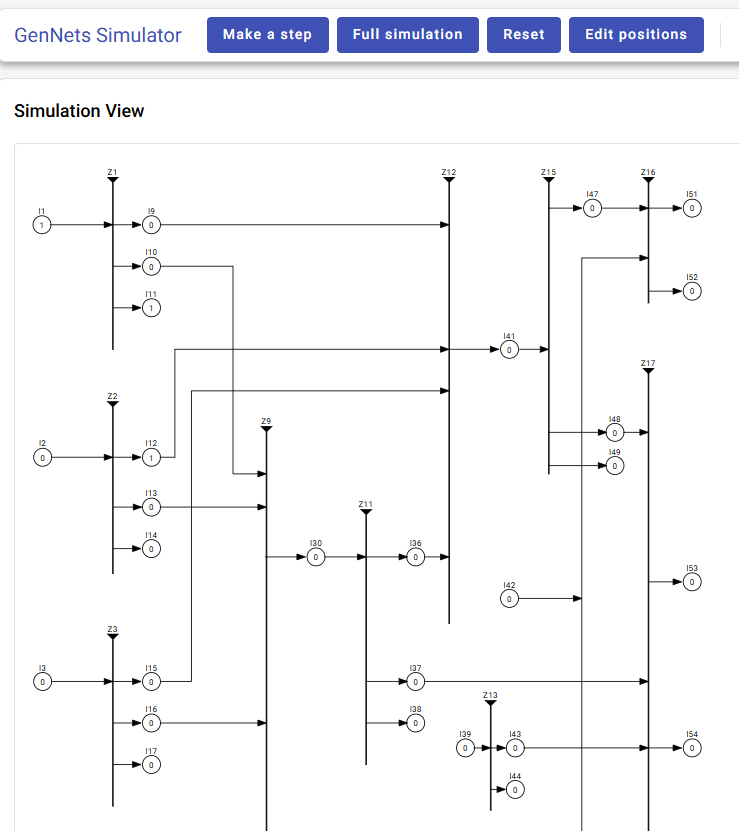
\includegraphics[width=1\linewidth]{4. applications/fuelGasEtc/images/upper.png}}
	\caption{Горна част на ОМ модела в \textit{OnlineGN}.}
	\label{fig:onlinegn-model-upper}
\end{figure}

\begin{figure}[H]
	\centering
	\setlength{\fboxrule}{2pt}
	\setlength{\fboxsep}{0pt}
	\fbox{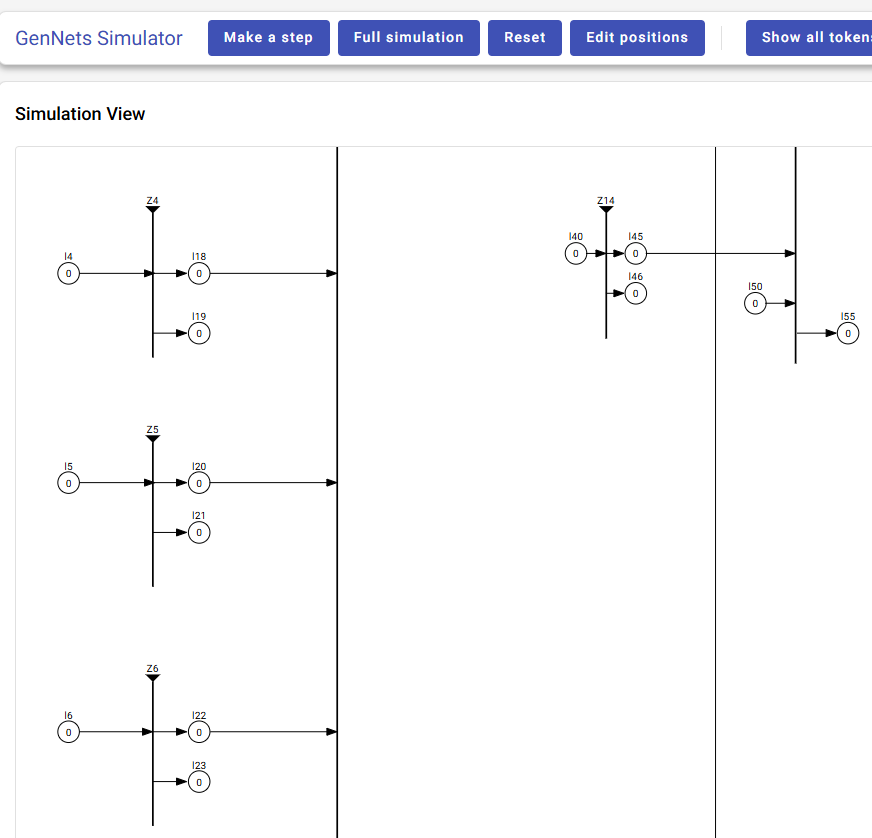
\includegraphics[width=1\linewidth]{4. applications/fuelGasEtc/images/middle.png}}
	\caption{Средна част на ОМ модела в \textit{OnlineGN}.}
	\label{fig:onlinegn-model-middle}
\end{figure}

\begin{figure}[H]
	\centering
	\setlength{\fboxrule}{2pt}
	\setlength{\fboxsep}{0pt}
	\fbox{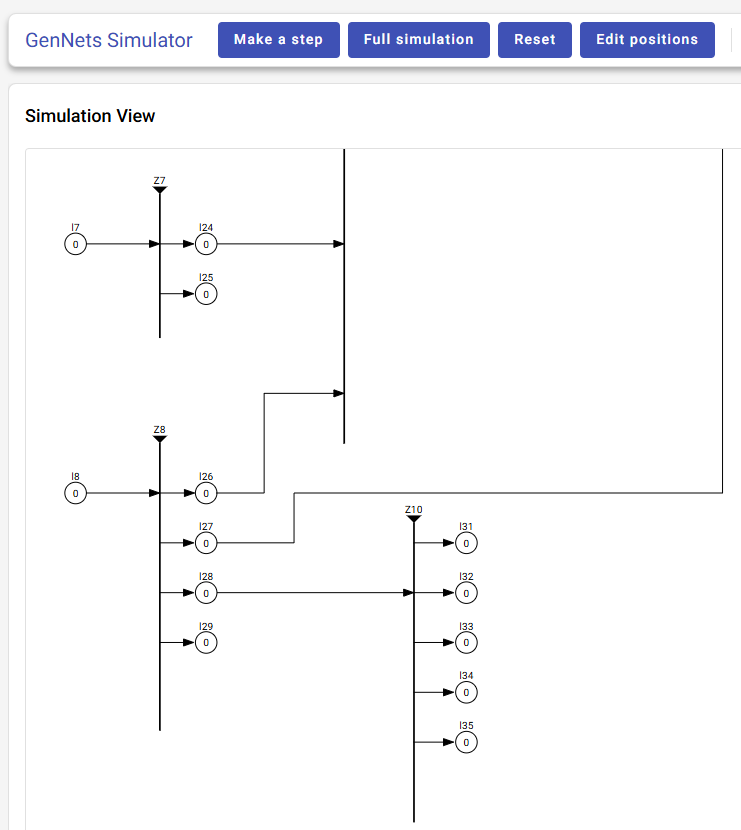
\includegraphics[width=1\linewidth]{4. applications/fuelGasEtc/images/bottom.png}}
	\caption{Долна част на ОМ модела в \textit{OnlineGN}.}
	\label{fig:onlinegn-model-lower}
\end{figure}

\vspace{0.4cm}

Следващата важна стъпка е логиката на преходите: за всеки преход са дефинирани индексирани матрици, в които са заложени предикатите от теоретичното описание. Именно тези предикати „решават“ дали дадено ядро може да премине от входните към изходните позиции на прехода. На \textbf{Фигура~\ref{fig:onlinegn-matrix-z1}} е показан пример с индексирана матрица за преход $Z_1$, който в модела съответства на \textit{CDU-2}.

\begin{figure}[H]
	\centering
	\setlength{\fboxrule}{2pt}
	\setlength{\fboxsep}{0pt}
	\fbox{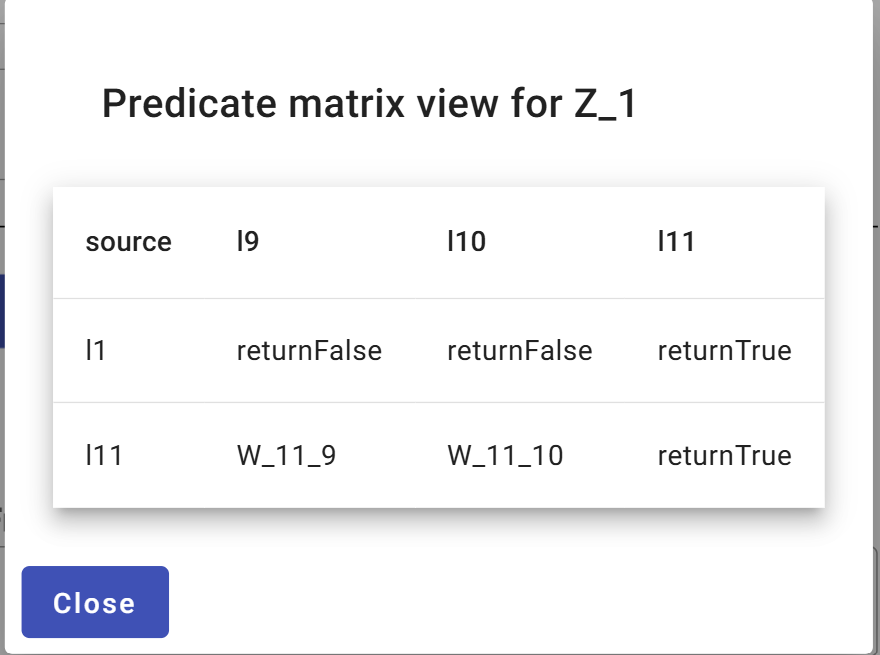
\includegraphics[width=0.5\linewidth]{4. applications/fuelGasEtc/images/matrix_1.png}}
	\captionsetup{width=0.8\textwidth}
	\caption{Индексирана матрица с предикатите за преход $Z_1$ (\textit{CDU-2}).}
	\label{fig:onlinegn-matrix-z1}
\end{figure}

В този конкретен пример предикатите отразяват условия от типа „има заявка за продукт ВПГ от \textit{CDU-2}“ и „има заявка за продукт горивен газ от \textit{CDU-2}“. С други думи, преходът $Z_1$ пропуска ядра нататък само когато са налице съответните заявки/условия, описани в модела.

Началните характеристики на ядрата са настроени според сценария от статията. На \textbf{Фигура~\ref{fig:onlinegn-token-l1}} е показано ядро във входната позиция $l_1$, което постъпва към $Z_1$ (\textit{CDU-2}), заедно с неговата начална характеристика. Тази характеристика съдържа необходимите атрибути за симулацията (например вид заявка и количества), така че по време на изпълнение да може ясно да се проследи какво „носи“ ядрото и какво се променя по веригата.

\begin{figure}[H]
	\centering
	\setlength{\fboxrule}{2pt}
	\setlength{\fboxsep}{0pt}
	\fbox{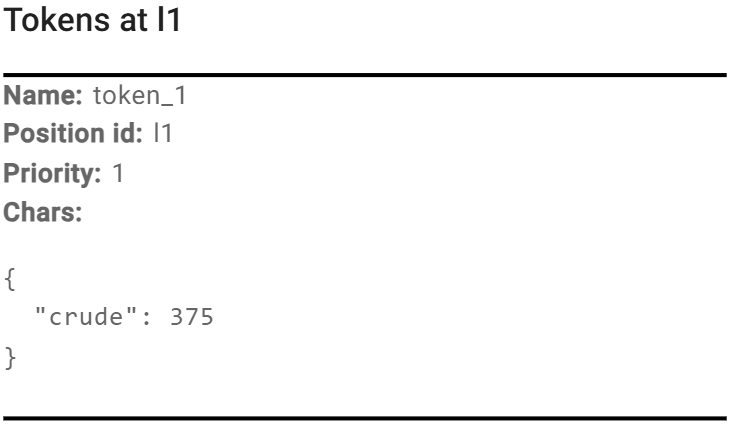
\includegraphics[width=0.5\linewidth]{4. applications/fuelGasEtc/images/token_1.png}}
	\captionsetup{width=0.8\textwidth}
	\caption{Ядро във входната позиция $l_1$ с начална характеристика (пример за вход към $Z_1$).}
	\label{fig:onlinegn-token-l1}
\end{figure}

След успешното изпълнение на симулацията наблюдаваните изходни характеристики съвпадат с очакваните теоретични резултати. Като конкретна илюстрация, на изходната позиция $l_{53}$ (обозначена като \textit{„LPG TANKS“}) се получава ядро, чиято характеристика съдържа количеството ВПГ, което моделът предвижда. Това е показано на \textbf{Фигура~\ref{fig:onlinegn-token-l53}}.

\begin{figure}[H]
	\centering
	\setlength{\fboxrule}{2pt}
	\setlength{\fboxsep}{0pt}
	\fbox{
\includegraphics[width=0.5\linewidth]{4. applications/fuelGasEtc/images/token_2.png}}
	\captionsetup{width=0.8\textwidth}
	\caption{Ядро в изходната позиция $l_{53}$ (\textit{„LPG TANKS“}) с характеристика след симулация.}
	\label{fig:onlinegn-token-l53}
\end{figure}

Обобщено, симулационните резултати потвърждават, че зададените предикати и начални характеристики работят коректно и че ОМ моделът описва адекватно разглеждания производствен процес. Това дава основание да приемем модела за валидиран спрямо теоретичния сценарий и използваем за последващи експерименти и анализи.


\subsubsection{Изводи за модела и симулацията}

\hspace*{2.5em}Процесът на производство на газообразни продукти в нефтопреработвателна рафинерия -- като газово гориво, пропан-бутан (Втечнен петролен газ, ВПГ) и пропилен, които могат да се експортират като готов краен продукт или да се използват като суровина за производство на полипропилен -- представлява сложен паралелен процес, чието описание чрез линейно, а често и чрез динамично програмиране е затруднено. Основната трудност е свързана с коректното отразяване на логиката на причинно--следствените връзки, която в ОМ се задава естествено чрез предикатите на преходните условия.

Настоящата глава представя ОМ модел за производството на газово гориво, ВПГ, пропилен и полипропилен в нефтопреработвателна рафинерия, както и неговата програмна реализация и симулация. Симулацията с \textit{OnlineGN} и получаването на резултати, съответстващи на очакваното поведение на процеса, потвърждават коректността на модела и демонстрират приложимостта на ОМ при моделиране и симулация на подобни производствени вериги.
